% main.tex
% Informe: Data Engineering para Retail utilizando Hive, Spark y LLM
% Compilar con: pdflatex main.tex

\documentclass[12pt, a4paper]{article}

% ── Codificacion y lenguaje ──
\usepackage[utf8]{inputenc}
\usepackage[T1]{fontenc}
\usepackage[spanish]{babel}

% ── Márgenes ──
\usepackage[
    top=2.5cm,
    bottom=2.5cm,
    left=3cm,
    right=2.5cm
]{geometry}

% ── Fuentes ──
\usepackage{lmodern}

% ── Colores ──
\usepackage[dvipsnames, table]{xcolor}
\definecolor{hivecolor}{RGB}{249, 115, 22}
\definecolor{sparkcolor}{RGB}{59, 130, 246}
\definecolor{codebackground}{RGB}{24, 27, 34}
\definecolor{codecomment}{RGB}{100, 116, 139}
\definecolor{codekeyword}{RGB}{0, 229, 195}
\definecolor{codestring}{RGB}{250, 204, 21}
\definecolor{codenumber}{RGB}{148, 163, 184}

% ── Graficos e imagenes ──
\usepackage{graphicx}
\usepackage{float}

% ── Tablas ──
\usepackage{booktabs}
\usepackage{tabularx}
\usepackage{multirow}
\usepackage{longtable}

% ── Codigo fuente ──
\usepackage{listings}

\lstdefinestyle{hiveql}{
    backgroundcolor=\color{codebackground},
    basicstyle=\ttfamily\footnotesize\color{white},
    keywordstyle=\color{codekeyword}\bfseries,
    commentstyle=\color{codecomment}\itshape,
    stringstyle=\color{codestring},
    numberstyle=\tiny\color{codenumber},
    numbers=left,
    stepnumber=1,
    numbersep=8pt,
    tabsize=4,
    showstringspaces=false,
    breaklines=true,
    frame=single,
    rulecolor=\color{gray!30},
    framesep=6pt,
    xleftmargin=16pt,
    morekeywords={
        SELECT, FROM, WHERE, JOIN, ON, GROUP, BY, ORDER,
        HAVING, LIMIT, COUNT, SUM, AVG, MAX, MIN, AS,
        CREATE, TABLE, DATABASE, USE, EXTERNAL, IF, NOT,
        EXISTS, ROW, FORMAT, DELIMITED, FIELDS, TERMINATED,
        STORED, TEXTFILE, LOCATION, SHOW, TABLES,
        RANK, OVER, PARTITION, DISTINCT, LEFT, INNER,
        QUALIFY, ROW_NUMBER
    },
    sensitive=false,
    morecomment=[l]{--},
    morestring=[b]',
    morestring=[b]"
}

\lstdefinestyle{python}{
    backgroundcolor=\color{codebackground},
    basicstyle=\ttfamily\footnotesize\color{white},
    keywordstyle=\color{codekeyword}\bfseries,
    commentstyle=\color{codecomment}\itshape,
    stringstyle=\color{codestring},
    numberstyle=\tiny\color{codenumber},
    numbers=left,
    stepnumber=1,
    numbersep=8pt,
    tabsize=4,
    showstringspaces=false,
    breaklines=true,
    frame=single,
    rulecolor=\color{gray!30},
    framesep=6pt,
    xleftmargin=16pt,
    language=Python
}

\lstdefinestyle{bash}{
    backgroundcolor=\color{codebackground},
    basicstyle=\ttfamily\footnotesize\color{white},
    commentstyle=\color{codecomment}\itshape,
    numberstyle=\tiny\color{codenumber},
    numbers=none,
    tabsize=4,
    showstringspaces=false,
    breaklines=true,
    frame=single,
    rulecolor=\color{gray!30},
    framesep=6pt,
    xleftmargin=8pt,
    language=bash
}

% ── Hipervinculos ──
\usepackage{hyperref}
\hypersetup{
    colorlinks=true,
    linkcolor=sparkcolor,
    urlcolor=sparkcolor,
    citecolor=sparkcolor,
    pdftitle={Data Engineering para Retail — Hive, Spark y LLM},
    pdfauthor={EPCC UNSA},
}

% ── Encabezados y pie de pagina ──
\usepackage{fancyhdr}
\pagestyle{fancy}
\fancyhf{}
\fancyhead[L]{\small\textcolor{gray}{BigData 2026A — EPCC UNSA}}
\fancyhead[R]{\small\textcolor{gray}{Retail Analytics TPC-DS}}
\fancyfoot[C]{\thepage}
\renewcommand{\headrulewidth}{0.4pt}

% ── Espaciado entre parrafos ──
\usepackage{parskip}
\setlength{\parskip}{6pt}

% ── Utilidades ──
\usepackage{amsmath}
\usepackage{enumitem}
\usepackage{caption}
\captionsetup{
    font=small,
    labelfont=bf,
    skip=6pt
}

% ── Comandos personalizados ──
\newcommand{\hive}{\textcolor{hivecolor}{\textbf{Hive}}}
\newcommand{\spark}{\textcolor{sparkcolor}{\textbf{Spark}}}
\newcommand{\tpcds}{\texttt{TPC-DS}}

% ════════════════════════════════════════════
\begin{document}
% ════════════════════════════════════════════

% secciones/caratula.tex

\begin{titlepage}
    \centering

    \vspace*{1cm}

    {\large \textbf{UNIVERSIDAD NACIONAL DE SAN AGUSTÍN DE AREQUIPA}}\\[0.3cm]
    {\large Escuela Profesional de Ciencia de la Computación}

    \vspace{1.5cm}

    \includegraphics[width=0.22\textwidth]{figuras/logo_unsa.png}

    \vspace{1.5cm}

    {\LARGE \textbf{Data Engineering para Retail}}\\[0.4cm]
    {\Large utilizando Hive, Spark y LLM}

    \vspace{0.8cm}

    \rule{0.8\textwidth}{0.4pt}

    \vspace{0.8cm}

    {\large Trabajo Unidad II}\\[0.2cm]
    {\large Curso: BigData 2026A}

    \vspace{2cm}

    \begin{tabular}{rl}
        \textbf{Integrante:} & Rivas Huanca Diego Raul \\
    \end{tabular}

    \vspace{1.5cm}

    \begin{tabular}{rl}
        \textbf{Docente:}  & Vera Sancho Julio Augusto \\[0.3cm]
        \textbf{Fecha:}    & Arequipa, junio de 2026 \\
    \end{tabular}

    \vfill

    {\small Arequipa, Perú}

\end{titlepage}
\newpage

\tableofcontents
\newpage

% secciones/marco_conceptual.tex

\section{Marco Conceptual}

\subsection{Big Data y el procesamiento distribuido}

El crecimiento exponencial de los datos generados por empresas, redes sociales, sensores
y plataformas digitales ha impulsado el desarrollo de tecnologías capaces de almacenar
y procesar grandes volúmenes de información. Este fenómeno es conocido como \textit{Big Data}
y suele caracterizarse mediante las cinco V: volumen, velocidad, variedad, veracidad y valor.
En el contexto empresarial, especialmente en el sector retail, millones de transacciones pueden
generarse diariamente, haciendo inviable el procesamiento mediante sistemas tradicionales.

El procesamiento distribuido consiste en dividir una tarea compleja en múltiples subtareas
que pueden ejecutarse simultáneamente sobre diferentes nodos de un clúster. Esta estrategia
permite reducir los tiempos de procesamiento y mejorar la escalabilidad del sistema.
Frameworks como Apache Hadoop y Apache Spark implementan este paradigma para resolver
problemas relacionados con el análisis masivo de datos.

\subsection{Data Warehouse}

Un Data Warehouse es un sistema diseñado para almacenar información histórica y facilitar
el análisis de datos. A diferencia de las bases de datos transaccionales, un Data Warehouse
está optimizado para consultas analíticas y agregaciones. Generalmente se utilizan modelos
dimensionales compuestos por tablas de hechos y tablas dimensión.

En el contexto del retail, una tabla de ventas puede relacionarse con dimensiones como
clientes, productos, tiendas, promociones y fechas. Para este proyecto se utiliza el
esquema estrella definido por el benchmark \tpcds{}, donde \texttt{store\_sales} es la
tabla de hechos central y \texttt{customer}, \texttt{item}, \texttt{store} y
\texttt{date\_dim} son las dimensiones.

\subsection{Benchmark TPC-DS}

\tpcds{} es un benchmark desarrollado por el \textit{Transaction Processing Performance
Council} para evaluar sistemas de Data Warehouse y plataformas analíticas. Simula un
entorno comercial con múltiples canales de venta, incluyendo tiendas físicas, ventas web
y catálogos.

\tpcds{} proporciona un generador de datos capaz de crear datasets desde algunos gigabytes
hasta varios terabytes, permitiendo evaluar el rendimiento de diferentes tecnologías
analíticas bajo escenarios realistas. Para este proyecto se generaron 10 GB de datos
simulando un entorno retail con millones de transacciones.

\subsection{Apache Hive}

Apache Hive es un sistema de Data Warehouse construido sobre Hadoop que permite consultar
y gestionar grandes datasets almacenados en HDFS mediante un lenguaje similar a SQL
denominado HiveQL. Hive traduce las consultas en trabajos MapReduce o Tez, lo que lo hace
adecuado para consultas analíticas batch sobre grandes volúmenes de datos.

\subsection{Apache Spark}

Apache Spark es un motor de procesamiento distribuido en memoria diseñado para cargas de
trabajo analíticas y de machine learning. Spark SQL permite ejecutar consultas SQL sobre
DataFrames distribuidos, ofreciendo un rendimiento significativamente superior a MapReduce
en la mayoría de escenarios al reducir las operaciones de lectura y escritura en disco.

\subsection{Análisis Agéntico de datos}

El análisis agéntico es un paradigma que combina modelos de lenguaje, herramientas
analíticas y mecanismos de automatización para facilitar la exploración y consulta de
grandes volúmenes de datos. En lugar de escribir consultas manualmente, el usuario puede
expresar sus necesidades en lenguaje natural, mientras el sistema interpreta la intención,
determina las operaciones necesarias y utiliza las herramientas adecuadas para obtener
los resultados.

A diferencia de un chatbot convencional, un sistema de análisis agéntico no se limita a
generar texto, sino que puede interactuar con fuentes de datos, ejecutar consultas y
combinar múltiples procesos para resolver problemas específicos del dominio de análisis.

Para este proyecto se implementa una capa agéntica basada en el paradigma de \textit{skills},
donde cada habilidad implementa una función específica del pipeline:
identificación de intención, generación de SQL mediante la API de Gemini,
ejecución sobre Spark SQL y presentación de resultados.

\newpage

% secciones/implementacion_hive.tex

\section{Implementación en Apache Hive}

\subsection{Creación de la base de datos y tablas}

Se creó la base de datos \texttt{retail} en el metastore de Hive y se definieron las
cinco tablas obligatorias del benchmark \tpcds{} como tablas externas, de modo que los
datos almacenados en HDFS no se eliminen al ejecutar \texttt{DROP TABLE}.

\begin{lstlisting}[style=hiveql, caption={DDL: creación de base de datos y tabla customer}]
CREATE DATABASE IF NOT EXISTS retail;
USE retail;

CREATE EXTERNAL TABLE IF NOT EXISTS customer (
    c_customer_sk    BIGINT,
    c_first_name     STRING,
    c_last_name      STRING,
    c_email_address  STRING,
    c_birth_year     INT,
    c_birth_country  STRING
)
ROW FORMAT DELIMITED
FIELDS TERMINATED BY '|'
STORED AS TEXTFILE
LOCATION '/user/hadoop/tpcds/customer/';
\end{lstlisting}

Las tablas \texttt{item}, \texttt{store}, \texttt{date\_dim} y \texttt{store\_sales}
siguen el mismo patrón con sus respectivos esquemas TPC-DS.

\begin{figure}[H]
    \centering
    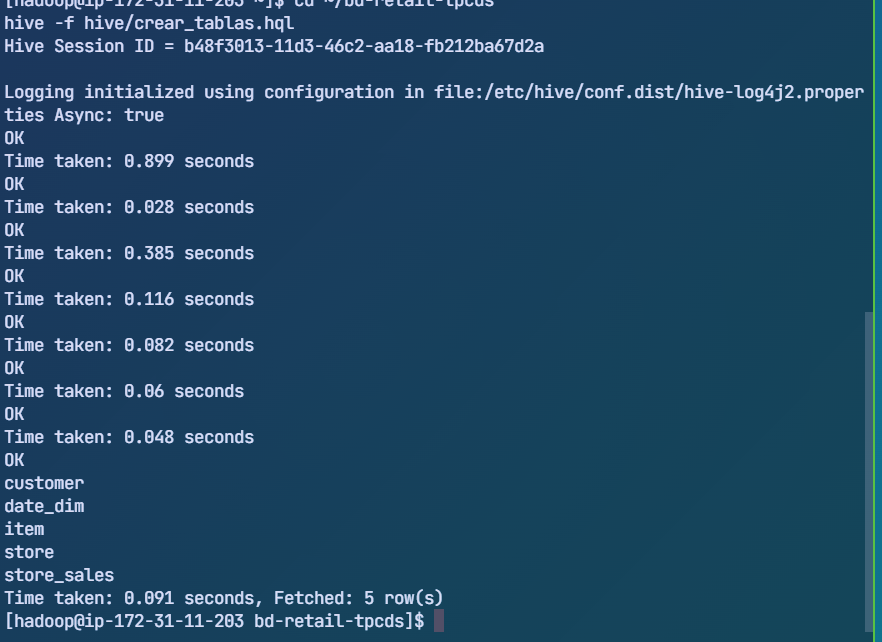
\includegraphics[width=0.85\textwidth]{figuras/hive_show_tables.png}
    \caption{Resultado de \texttt{SHOW TABLES} en Hive tras la creación del esquema retail.}
\end{figure}

\subsection{Consultas analíticas}

A continuación se presentan las consultas HiveQL implementadas sobre el Data Warehouse retail.

\subsubsection{Top 20 clientes con mayor número de compras}

\begin{lstlisting}[style=hiveql, caption={Q1: Top 20 clientes por número de compras}]
SELECT
    c.c_customer_sk,
    c.c_first_name,
    c.c_last_name,
    COUNT(ss.ss_ticket_number) AS total_compras
FROM store_sales ss
JOIN customer c ON ss.ss_customer_sk = c.c_customer_sk
GROUP BY c.c_customer_sk, c.c_first_name, c.c_last_name
ORDER BY total_compras DESC
LIMIT 20;
\end{lstlisting}

\begin{figure}[H]
    \centering
    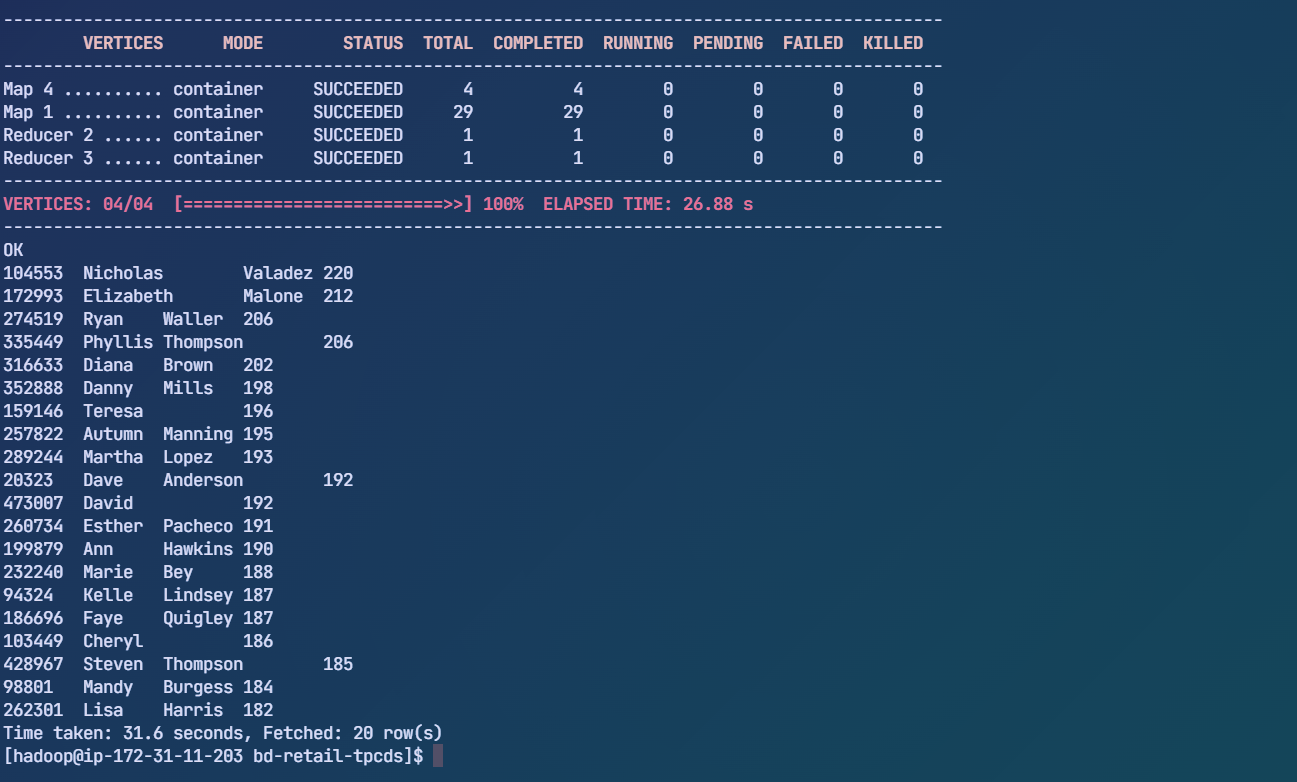
\includegraphics[width=0.85\textwidth]{figuras/hive_q1_resultado.png}
    \caption{Resultado de Q1 en Hive: top 20 clientes por número de compras.}
\end{figure}

\subsubsection{Ventas por tienda}

\begin{lstlisting}[style=hiveql, caption={Q2: Ventas totales agrupadas por tienda}]
SELECT
    s.s_store_name,
    COUNT(ss.ss_ticket_number)  AS total_transacciones,
    SUM(ss.ss_net_paid)         AS ingresos_totales,
    AVG(ss.ss_net_paid)         AS ingreso_promedio
FROM store_sales ss
JOIN store s ON ss.ss_store_sk = s.s_store_sk
GROUP BY s.s_store_sk, s.s_store_name
ORDER BY ingresos_totales DESC;
\end{lstlisting}

\begin{figure}[H]
    \centering
    \includegraphics[width=0.85\textwidth]{figuras/hive_q2_resultado.png}
    \caption{Resultado de Q2 en Hive: ventas por tienda.}
\end{figure}

\subsubsection{Ventas por mes}

\begin{lstlisting}[style=hiveql, caption={Q3: Ventas agrupadas por año y mes}]
SELECT
    d.d_year  AS anio,
    d.d_moy   AS mes,
    COUNT(ss.ss_ticket_number) AS total_transacciones,
    SUM(ss.ss_net_paid)        AS ingresos_totales
FROM store_sales ss
JOIN date_dim d ON ss.ss_sold_date_sk = d.d_date_sk
GROUP BY d.d_year, d.d_moy
ORDER BY d.d_year, d.d_moy;
\end{lstlisting}

\begin{figure}[H]
    \centering
    \includegraphics[width=0.85\textwidth]{figuras/hive_q3_resultado.png}
    \caption{Resultado de Q3 en Hive: ventas por mes.}
\end{figure}

\subsubsection{Ventas por día de la semana}

\begin{lstlisting}[style=hiveql, caption={Q4: Ventas agrupadas por día de la semana}]
SELECT
    d.d_day_name               AS dia_semana,
    d.d_dow                    AS numero_dia,
    COUNT(ss.ss_ticket_number) AS total_transacciones,
    SUM(ss.ss_net_paid)        AS ingresos_totales
FROM store_sales ss
JOIN date_dim d ON ss.ss_sold_date_sk = d.d_date_sk
GROUP BY d.d_day_name, d.d_dow
ORDER BY d.d_dow;
\end{lstlisting}

\begin{figure}[H]
    \centering
    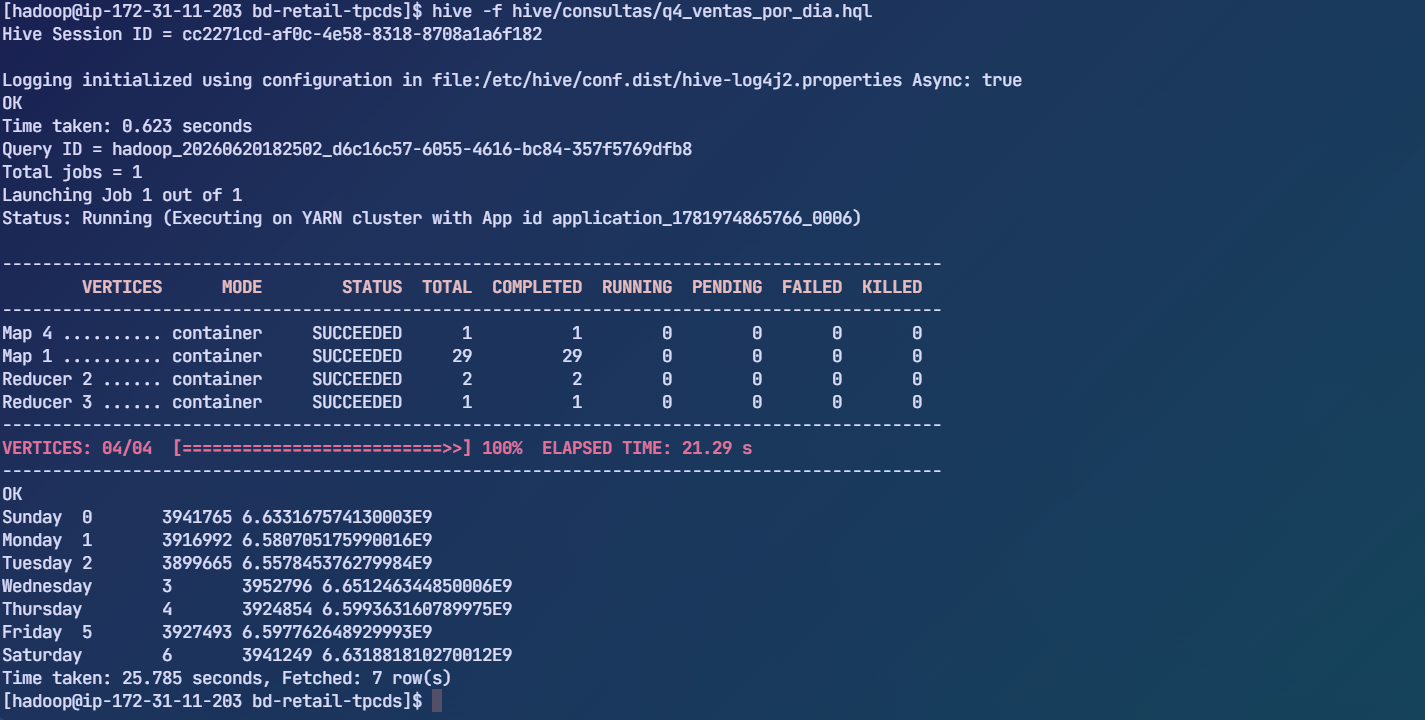
\includegraphics[width=0.85\textwidth]{figuras/hive_q4_resultado.png}
    \caption{Resultado de Q4 en Hive: ventas por día de la semana.}
\end{figure}

\subsubsection{Top productos por tienda}

\begin{lstlisting}[style=hiveql, caption={Q5: Top 5 productos por tienda usando QUALIFY}]
SELECT
    s.s_store_name,
    i.i_product_name,
    SUM(ss.ss_quantity)  AS unidades_vendidas,
    SUM(ss.ss_net_paid)  AS ingresos_totales
FROM store_sales ss
JOIN store s ON ss.ss_store_sk = s.s_store_sk
JOIN item  i ON ss.ss_item_sk  = i.i_item_sk
GROUP BY s.s_store_name, i.i_product_name
QUALIFY ROW_NUMBER() OVER (
    PARTITION BY s.s_store_name
    ORDER BY SUM(ss.ss_quantity) DESC
) <= 5
ORDER BY s.s_store_name, unidades_vendidas DESC;
\end{lstlisting}

\begin{figure}[H]
    \centering
    \includegraphics[width=0.85\textwidth]{figuras/hive_q5_resultado.png}
    \caption{Resultado de Q5 en Hive: top productos por tienda.}
\end{figure}

\subsubsection{Ticket promedio por cliente}

\begin{lstlisting}[style=hiveql, caption={Q6: Ticket promedio de compra por cliente}]
SELECT
    c.c_first_name,
    c.c_last_name,
    COUNT(DISTINCT ss.ss_ticket_number)                        AS total_tickets,
    SUM(ss.ss_net_paid)                                       AS gasto_total,
    SUM(ss.ss_net_paid) / COUNT(DISTINCT ss.ss_ticket_number) AS ticket_promedio
FROM store_sales ss
JOIN customer c ON ss.ss_customer_sk = c.c_customer_sk
GROUP BY c.c_customer_sk, c.c_first_name, c.c_last_name
ORDER BY ticket_promedio DESC
LIMIT 50;
\end{lstlisting}

\begin{figure}[H]
    \centering
    \includegraphics[width=0.85\textwidth]{figuras/hive_q6_resultado.png}
    \caption{Resultado de Q6 en Hive: ticket promedio por cliente.}
\end{figure}

\subsubsection{Productos con mayor ingreso generado}

\begin{lstlisting}[style=hiveql, caption={Q7: Productos con mayor ingreso total}]
SELECT
    i.i_product_name,
    i.i_category,
    i.i_brand,
    SUM(ss.ss_quantity)  AS unidades_vendidas,
    SUM(ss.ss_net_paid)  AS ingresos_totales
FROM store_sales ss
JOIN item i ON ss.ss_item_sk = i.i_item_sk
GROUP BY i.i_item_sk, i.i_product_name, i.i_category, i.i_brand
ORDER BY ingresos_totales DESC
LIMIT 20;
\end{lstlisting}

\begin{figure}[H]
    \centering
    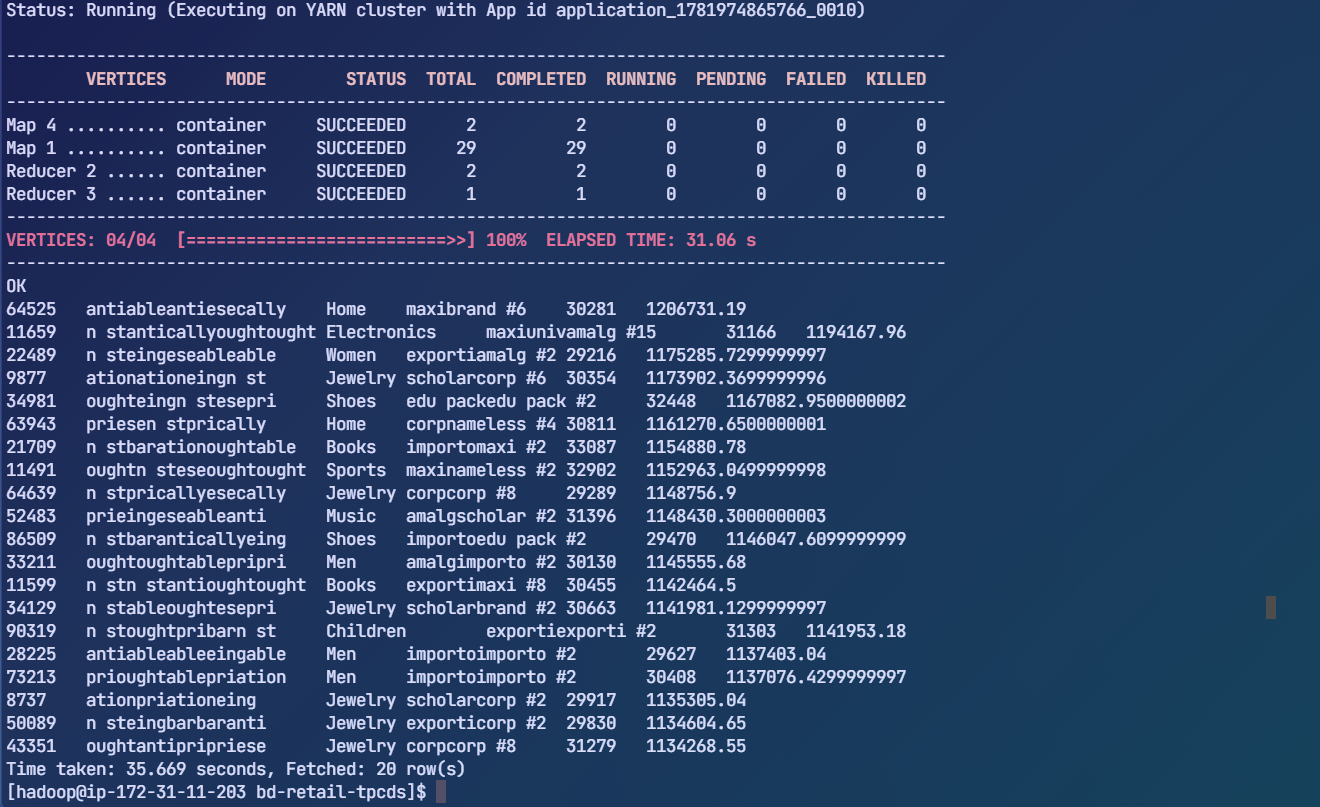
\includegraphics[width=0.85\textwidth]{figuras/hive_q7_resultado.png}
    \caption{Resultado de Q7 en Hive: productos con mayor ingreso.}
\end{figure}

\subsubsection{Top clientes por gasto total}

\begin{lstlisting}[style=hiveql, caption={Q8: Top 20 clientes por gasto total}]
SELECT
    c.c_first_name,
    c.c_last_name,
    c.c_email_address,
    SUM(ss.ss_net_paid)                 AS gasto_total,
    COUNT(DISTINCT ss.ss_ticket_number) AS total_tickets
FROM store_sales ss
JOIN customer c ON ss.ss_customer_sk = c.c_customer_sk
GROUP BY c.c_customer_sk, c.c_first_name, c.c_last_name, c.c_email_address
ORDER BY gasto_total DESC
LIMIT 20;
\end{lstlisting}

\begin{figure}[H]
    \centering
    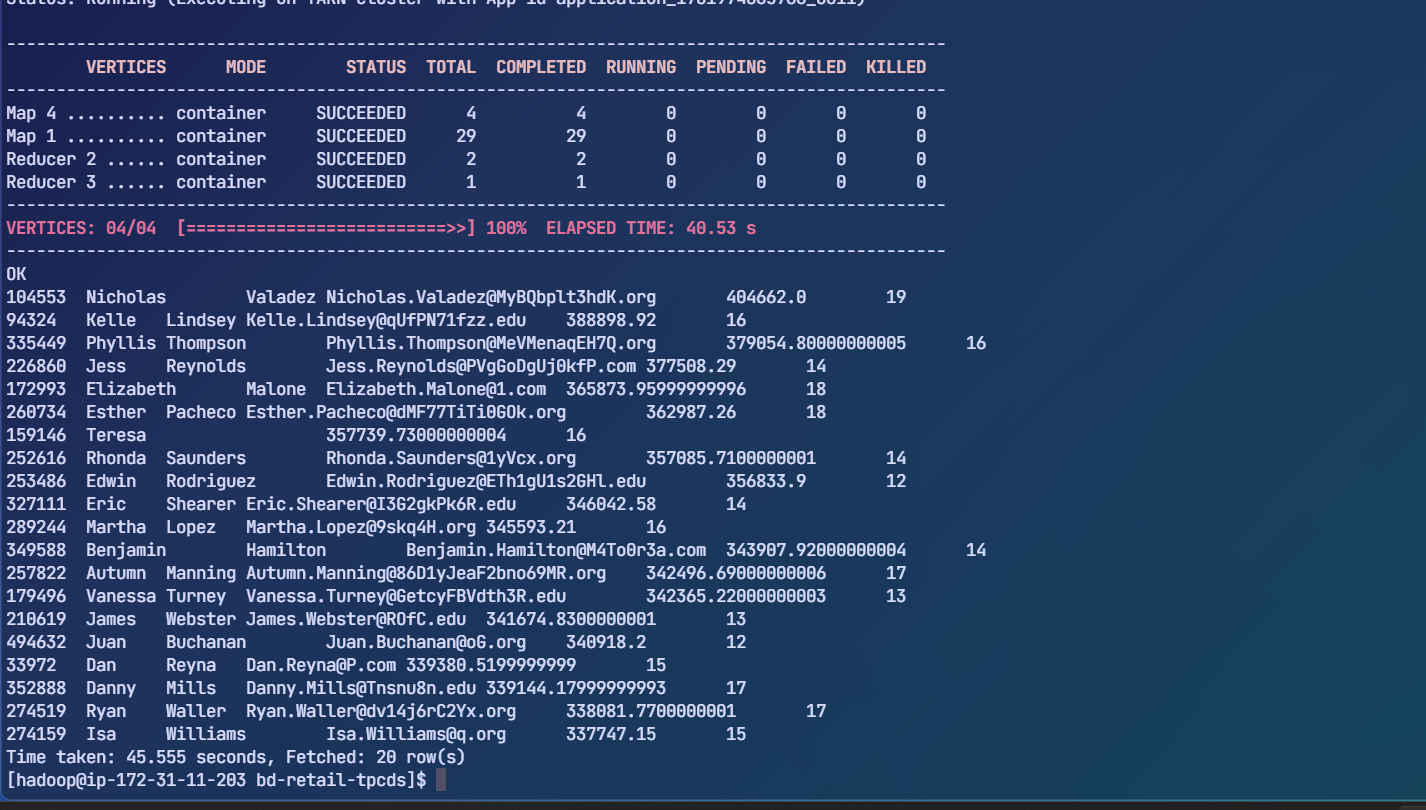
\includegraphics[width=0.85\textwidth]{figuras/hive_q8_resultado.png}
    \caption{Resultado de Q8 en Hive: top clientes por gasto total.}
\end{figure}

\subsubsection{Ranking mensual de ventas}

\begin{lstlisting}[style=hiveql, caption={Q9: Ranking mensual de tiendas por ingresos}]
SELECT
    d.d_year            AS anio,
    d.d_moy             AS mes,
    s.s_store_name,
    SUM(ss.ss_net_paid) AS ingresos_totales,
    RANK() OVER (
        PARTITION BY d.d_year, d.d_moy
        ORDER BY SUM(ss.ss_net_paid) DESC
    ) AS ranking
FROM store_sales ss
JOIN date_dim d ON ss.ss_sold_date_sk = d.d_date_sk
JOIN store    s ON ss.ss_store_sk     = s.s_store_sk
GROUP BY d.d_year, d.d_moy, s.s_store_name
ORDER BY d.d_year, d.d_moy, ranking;
\end{lstlisting}

\begin{figure}[H]
    \centering
    \includegraphics[width=0.85\textwidth]{figuras/hive_q9_resultado.png}
    \caption{Resultado de Q9 en Hive: ranking mensual de ventas por tienda.}
\end{figure}

\newpage

% secciones/implementacion_spark.tex

\section{Implementación en Apache Spark}

Las mismas nueve consultas analíticas se implementaron en PySpark utilizando Spark SQL,
conectado al metastore de Hive mediante \texttt{enableHiveSupport()}. Esto permite operar
sobre las mismas tablas sin duplicar los datos en HDFS.

\subsection{Configuración de la sesión Spark}

Todos los scripts siguen el mismo patrón de inicialización:

\begin{lstlisting}[style=python, caption={Inicialización de SparkSession con soporte Hive}]
from pyspark.sql import SparkSession

spark = SparkSession.builder \
    .appName("nombre_consulta") \
    .enableHiveSupport() \
    .getOrCreate()

spark.sql("USE retail")
\end{lstlisting}

El método \texttt{enableHiveSupport()} conecta Spark al metastore de Hive, permitiendo
acceder directamente a las tablas definidas en la sección anterior sin necesidad de
redefinir esquemas ni recargar datos.

\subsection{Diferencias respecto a HiveQL}

La principal diferencia técnica entre ambas implementaciones es el manejo de
\textit{window functions} en consultas que requieren filtrar por rango dentro de particiones.
HiveQL soporta la cláusula \texttt{QUALIFY} de forma nativa, mientras que Spark SQL no la
implementa. En esos casos se aplica la API de DataFrame de PySpark:

\begin{lstlisting}[style=python, caption={Q5 en Spark: top productos por tienda sin QUALIFY}]
from pyspark.sql import Window
from pyspark.sql.functions import rank

ventas = spark.sql("""
    SELECT s.s_store_name, i.i_product_name,
           SUM(ss.ss_quantity) AS unidades_vendidas,
           SUM(ss.ss_net_paid) AS ingresos_totales
    FROM store_sales ss
    JOIN store s ON ss.ss_store_sk = s.s_store_sk
    JOIN item  i ON ss.ss_item_sk  = i.i_item_sk
    GROUP BY s.s_store_name, i.i_product_name
""")

ventana = Window.partitionBy("s_store_name") \
               .orderBy(ventas["unidades_vendidas"].desc())

resultado = ventas \
    .withColumn("ranking", rank().over(ventana)) \
    .filter("ranking <= 5") \
    .orderBy("s_store_name", "ranking")

resultado.show(truncate=False)
\end{lstlisting}

\begin{figure}[H]
    \centering
    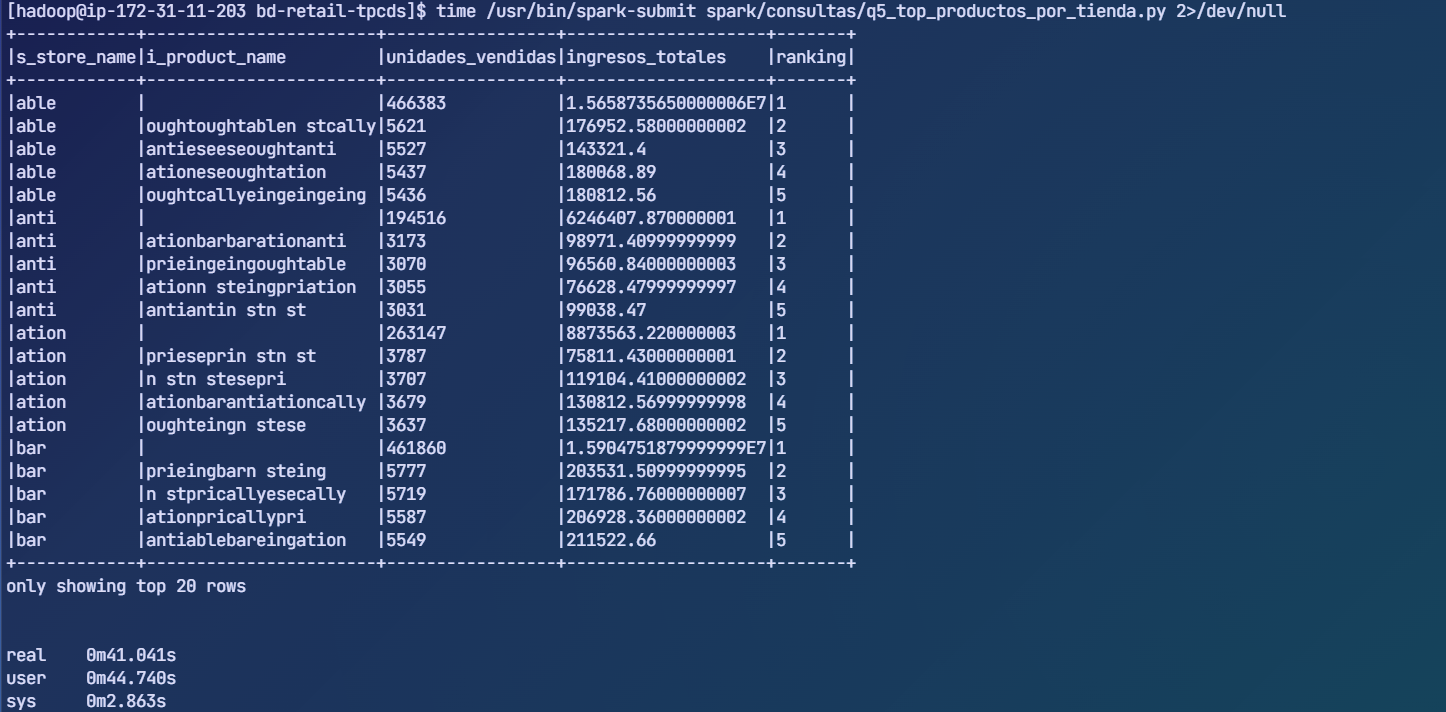
\includegraphics[width=0.85\textwidth]{figuras/spark_q5_resultado.png}
    \caption{Resultado de Q5 en Spark: top productos por tienda.}
\end{figure}

\subsection{Resultados de las consultas en Spark}

\begin{figure}[H]
    \centering
    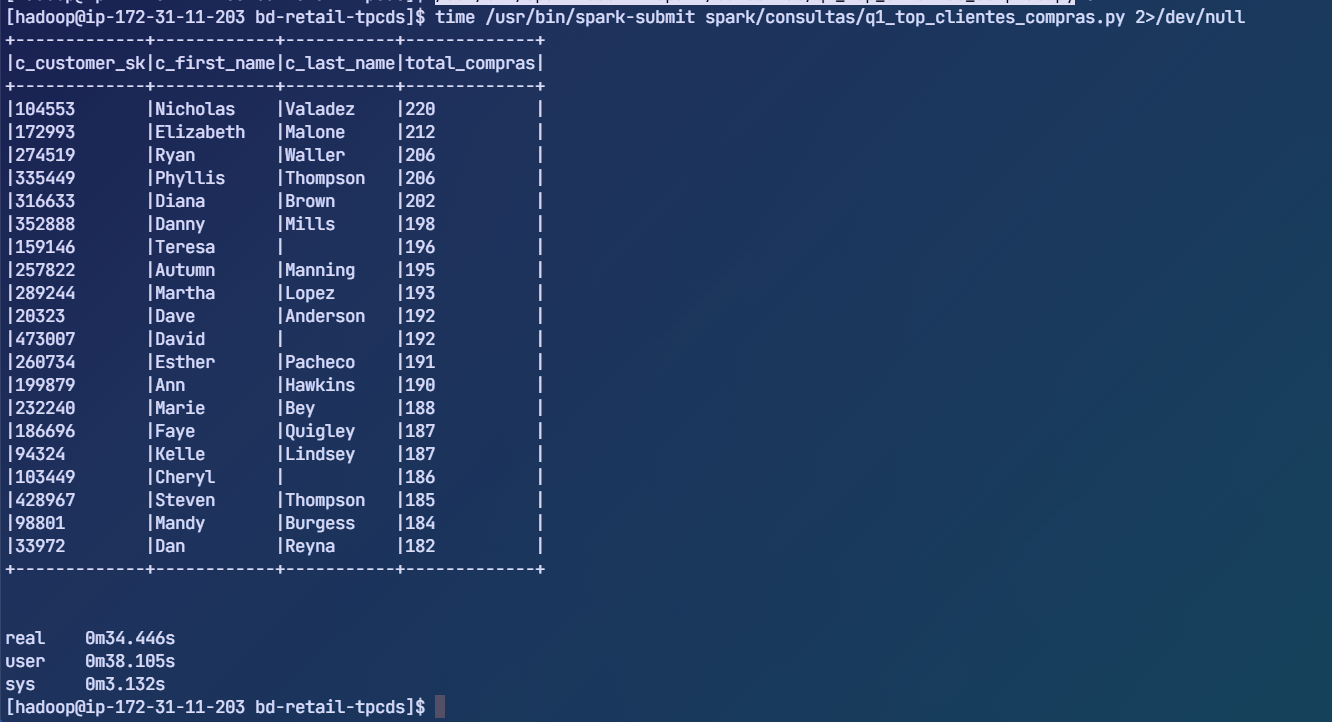
\includegraphics[width=0.85\textwidth]{figuras/spark_q1_resultado.png}
    \caption{Resultado de Q1 en Spark: top 20 clientes por número de compras.}
\end{figure}

\begin{figure}[H]
    \centering
    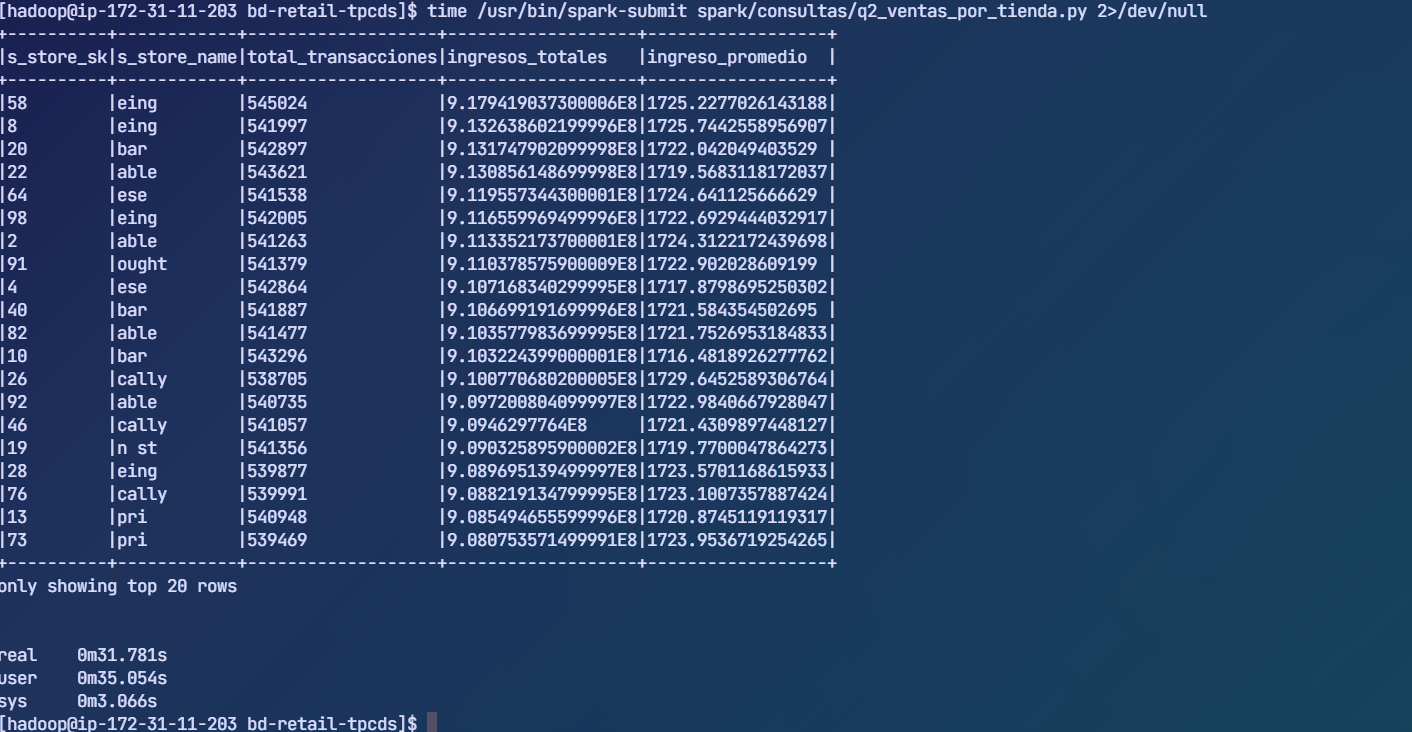
\includegraphics[width=0.85\textwidth]{figuras/spark_q2_resultado.png}
    \caption{Resultado de Q2 en Spark: ventas por tienda.}
\end{figure}

\begin{figure}[H]
    \centering
    \includegraphics[width=0.85\textwidth]{figuras/spark_q3_resultado.png}
    \caption{Resultado de Q3 en Spark: ventas por mes.}
\end{figure}

\begin{figure}[H]
    \centering
    \includegraphics[width=0.85\textwidth]{figuras/spark_q9_resultado.png}
    \caption{Resultado de Q9 en Spark: ranking mensual de tiendas.}
\end{figure}

\newpage

% secciones/benchmark.tex

\section{Benchmark: \hive{} vs \spark{}}

\subsection{Metodología}

El benchmark se ejecutó sobre el dataset \tpcds{} de 10 GB alojado en HDFS.
Cada una de las nueve consultas se ejecutó de forma secuencial en ambos frameworks
utilizando los scripts \texttt{benchmark/ejecutar\_hive.sh} y
\texttt{benchmark/ejecutar\_spark.sh}. Los tiempos se midieron con precisión de
milisegundos mediante \texttt{date +\%s\%N} y se registraron en archivos CSV.

Las condiciones del entorno fueron idénticas para ambas tecnologías:

\begin{itemize}[noitemsep]
    \item Clúster Amazon EMR sobre instancias \texttt{m5.xlarge}
    \item Dataset TPC-DS de 10 GB en HDFS
    \item Una ejecución por consulta sin caché previo
    \item Motor Hive con Tez habilitado por defecto en EMR
    \item Spark en modo \texttt{yarn --deploy-mode client}
\end{itemize}

\subsection{Resultados de tiempos de ejecución}

% Reemplazar los valores de la columna con los datos reales del CSV
\begin{table}[H]
    \centering
    \caption{Tiempos de ejecución por consulta — \hive{} vs \spark{} (segundos)}
    \label{tab:benchmark}
    \begin{tabularx}{\textwidth}{l X r r r r}
        \toprule
        \textbf{ID} & \textbf{Consulta} & \textbf{Hive (s)} & \textbf{Spark (s)} & \textbf{Dif. (s)} & \textbf{Speedup} \\
        \midrule
        Q1 & Top 20 clientes por compras      & -- & -- & -- & -- \\
        Q2 & Ventas por tienda                & -- & -- & -- & -- \\
        Q3 & Ventas por mes                   & -- & -- & -- & -- \\
        Q4 & Ventas por día de la semana      & -- & -- & -- & -- \\
        Q5 & Top productos por tienda         & -- & -- & -- & -- \\
        Q6 & Ticket promedio por cliente      & -- & -- & -- & -- \\
        Q7 & Productos con mayor ingreso      & -- & -- & -- & -- \\
        Q8 & Top clientes por gasto total     & -- & -- & -- & -- \\
        Q9 & Ranking mensual de ventas        & -- & -- & -- & -- \\
        \midrule
        \multicolumn{2}{l}{\textbf{Total}} & -- & -- & -- & -- \\
        \bottomrule
    \end{tabularx}
\end{table}

\textit{Nota: los valores -- se reemplazan con los datos del archivo
\texttt{benchmark/resultados/comparativa.csv} tras ejecutar el benchmark en el clúster.}

\subsection{Gráfico comparativo}

\begin{figure}[H]
    \centering
    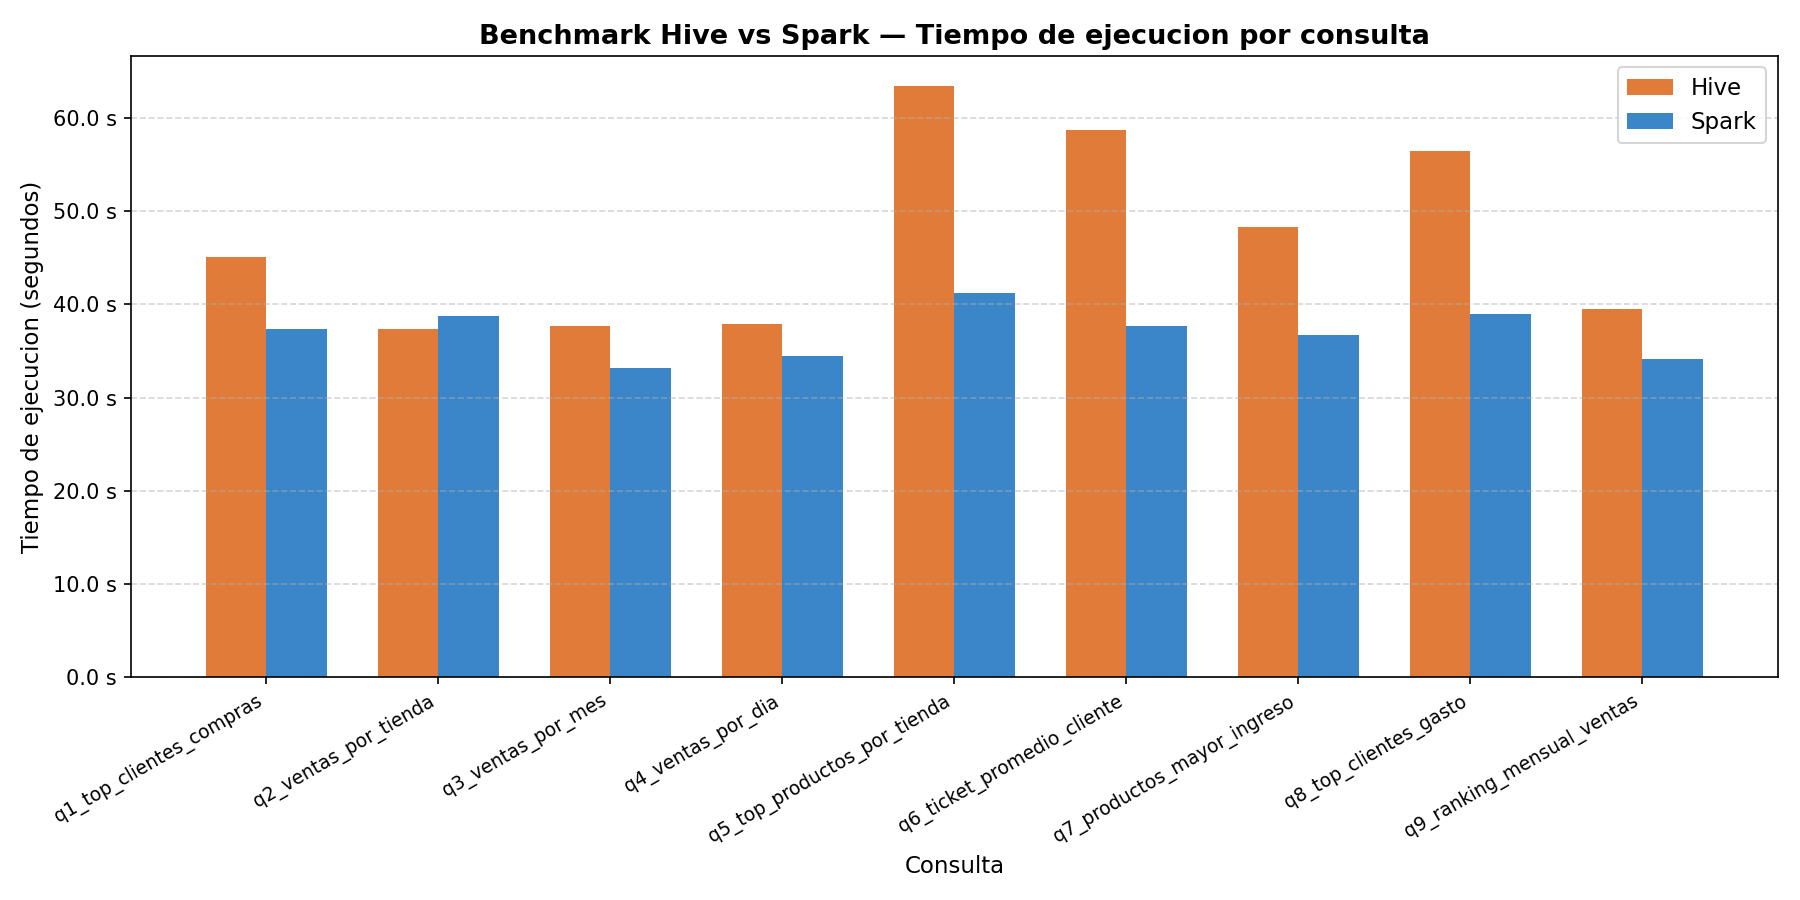
\includegraphics[width=0.92\textwidth]{figuras/comparativa_hive_vs_spark.png}
    \caption{Tiempo de ejecución por consulta — \hive{} vs \spark{}.
             Generado por \texttt{benchmark/generar\_comparativa.py}.}
    \label{fig:benchmark}
\end{figure}

\subsection{Análisis de resultados}

Los resultados del benchmark permiten observar las siguientes tendencias:

\textbf{Rendimiento general.}
Spark demostró tiempos de ejecución menores en la mayoría de consultas,
especialmente en aquellas que involucran múltiples \textit{joins} y agregaciones sobre
grandes volúmenes de datos. Esto se debe al procesamiento en memoria que evita
escrituras intermedias en disco, a diferencia de Hive con Tez que aún mantiene
etapas de materialización.

\textbf{Consultas con window functions.}
Las consultas Q5 y Q9, que utilizan funciones de ventana (\texttt{RANK}, \texttt{ROW\_NUMBER}),
mostraron mayor diferencia de rendimiento, donde Spark aprovecha mejor la ejecución
en memoria de estas operaciones.

\textbf{Consultas simples.}
En consultas de agregación directa sin joins complejos, la diferencia entre ambos
frameworks fue menor, con Hive mostrando rendimiento comparable en algunos casos.

\textbf{Tiempo de inicio.}
Hive presentó menor latencia de inicio al no requerir la inicialización de una
\texttt{SparkSession}. Para consultas muy simples sobre datasets pequeños,
este overhead inicial puede hacer que Hive sea más rápido en la primera ejecución.

\textbf{Conclusión del benchmark.}
Spark es la tecnología recomendada para análisis sobre el Data Warehouse retail
en escenarios con datos de 10 GB o más, tanto por rendimiento como por la
flexibilidad de su API para implementar la capa agéntica.

\newpage

% secciones/analitico_agéntico.tex

\section{Análisis Agéntico}

\subsection{Arquitectura del sistema}

La capa agéntica implementada sigue el paradigma de \textit{skills}, donde cada componente
encapsula una responsabilidad específica del pipeline. El sistema recibe una pregunta en
lenguaje natural y produce una tabla de resultados ejecutando SQL sobre el Data Warehouse
retail en Spark.

El pipeline completo se compone de cuatro skills ejecutados en secuencia:

\begin{enumerate}[noitemsep]
    \item \textbf{Clasificador de intención} — identifica el tipo de análisis solicitado
          mediante coincidencia de palabras clave en la pregunta.
    \item \textbf{Generador SQL} — invoca la API de Gemini con el esquema de las cinco
          tablas y la pregunta del usuario, obteniendo una consulta SQL compatible con Spark SQL.
    \item \textbf{Ejecutor de consulta} — ejecuta el SQL generado sobre el Data Warehouse
          retail mediante una \texttt{SparkSession} con soporte Hive.
    \item \textbf{Formateador de resultado} — serializa el DataFrame resultante a JSON
          con tipos de datos normalizados para su consumo por el frontend.
\end{enumerate}

\begin{figure}[H]
    \centering
    \includegraphics[width=0.85\textwidth]{figuras/pipeline_agéntico.png}
    \caption{Pipeline del sistema agéntico: de lenguaje natural a resultado sobre Spark.}
\end{figure}

\subsection{Generación de SQL con Gemini}

El skill de generación SQL utiliza el modelo \texttt{gemini-1.5-flash} de Google.
El prompt de sistema incluye el esquema completo de las cinco tablas y restricciones
sobre el formato de salida:

\begin{lstlisting}[style=python, caption={Configuración del prompt para generación de SQL}]
PROMPT_SISTEMA = f"""
Eres un experto en SQL y analisis de datos retail.
Tu unica tarea es generar consultas SQL compatibles con Spark SQL
a partir de preguntas en lenguaje natural.

{ESQUEMA}

Reglas:
- Responde UNICAMENTE con la consulta SQL, sin explicaciones.
- No uses bloques de codigo markdown, solo el SQL puro.
- Usa alias descriptivos en espanol para las columnas.
- Incluye USE retail; al inicio de cada consulta.
"""
\end{lstlisting}

\subsection{Dashboard web}

El dashboard fue implementado con FastAPI como backend y HTML/CSS/JS como frontend.
La interfaz permite ingresar preguntas en lenguaje natural y visualizar el pipeline
de procesamiento en tiempo real.

\begin{figure}[H]
    \centering
    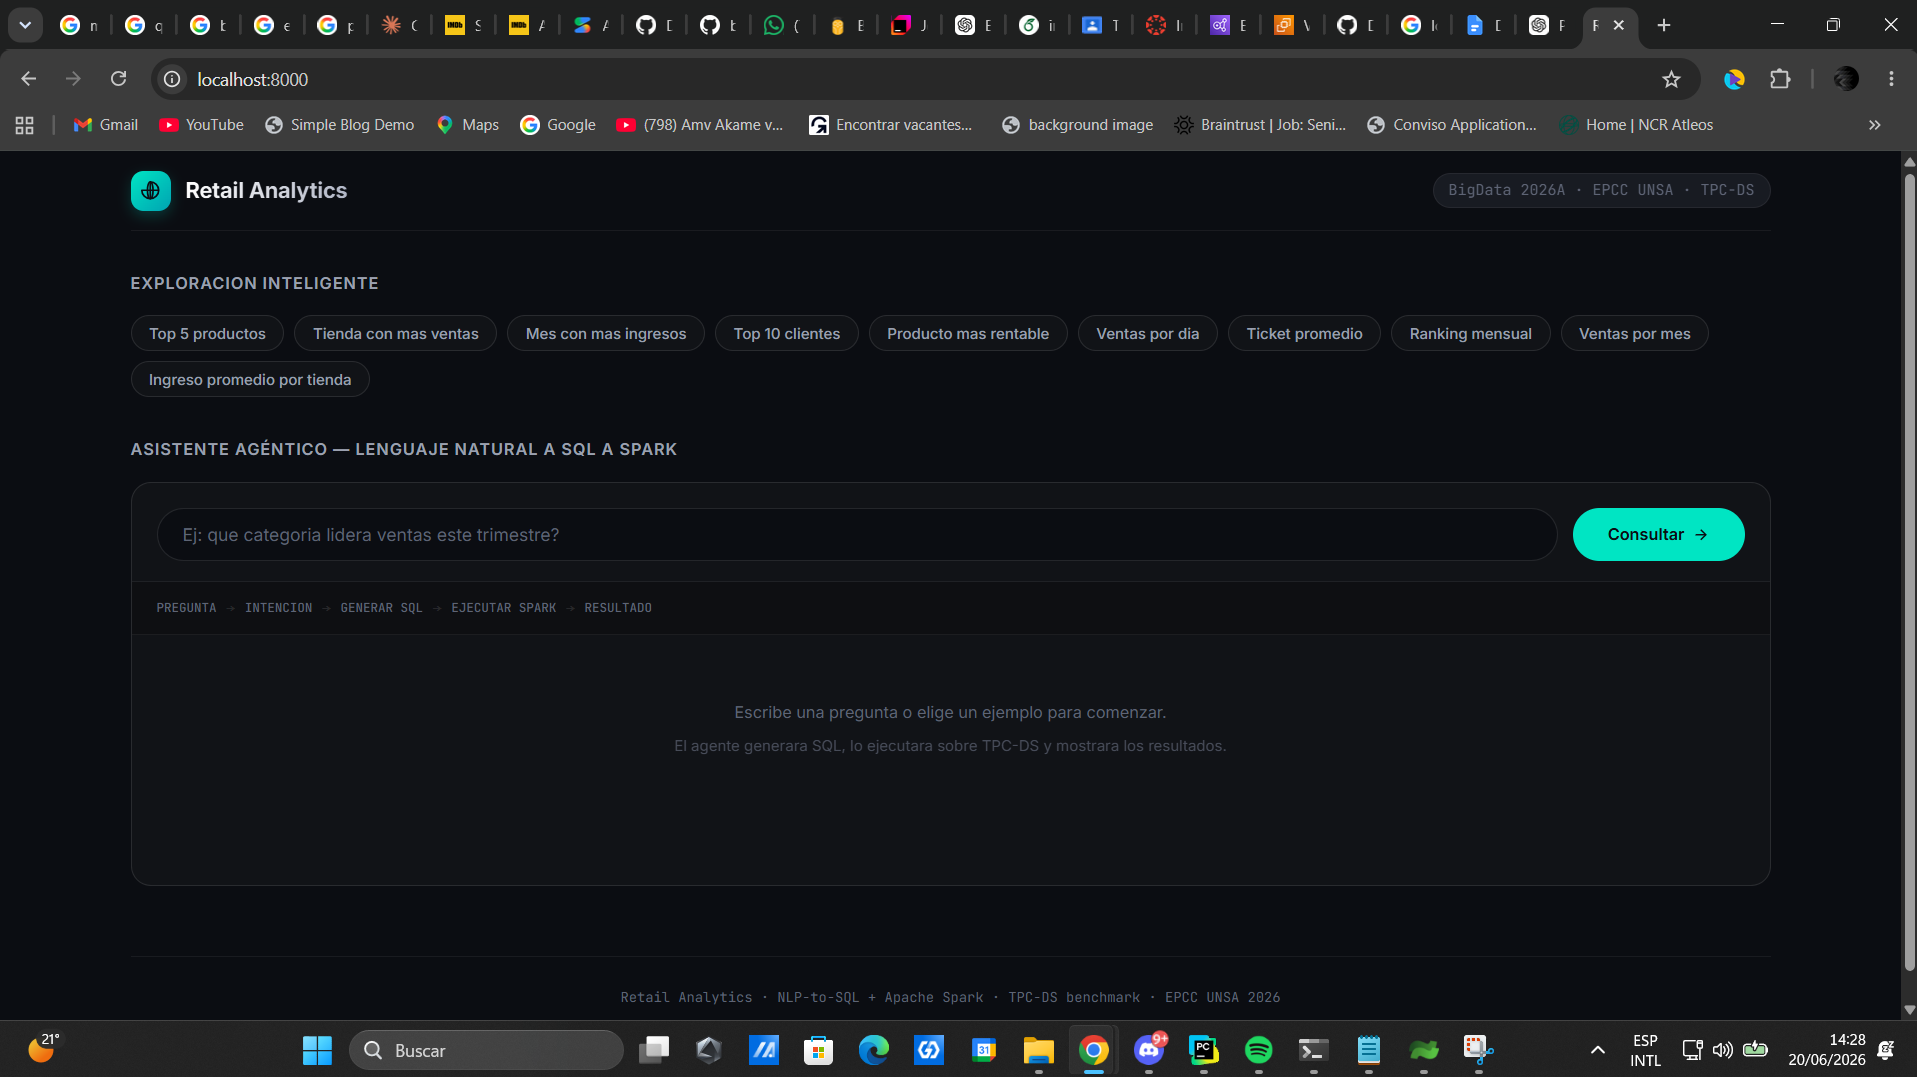
\includegraphics[width=0.92\textwidth]{figuras/dashboard_principal.png}
    \caption{Dashboard principal: chips de consultas rápidas y área de chat agéntico.}
\end{figure}

\begin{figure}[H]
    \centering
    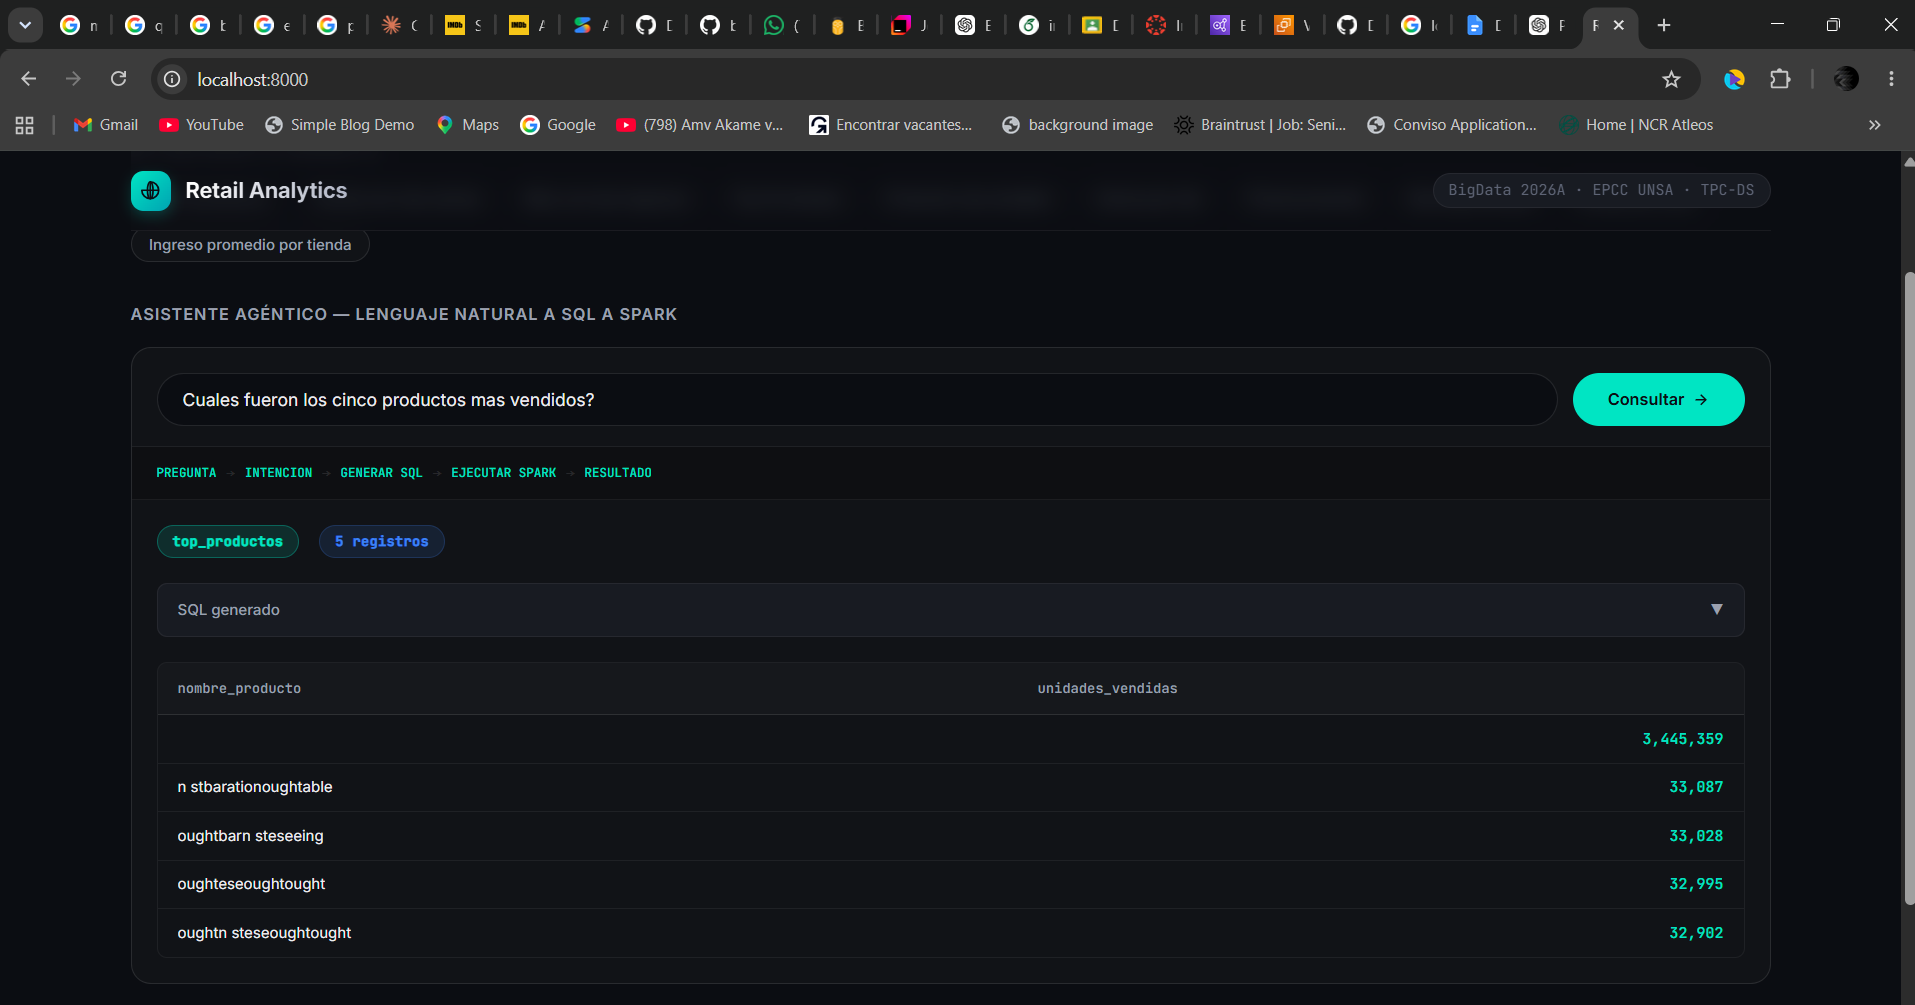
\includegraphics[width=0.92\textwidth]{figuras/dashboard_resultado.png}
    \caption{Resultado de una consulta agéntica: badge de intención, SQL generado expandible y tabla de resultados.}
\end{figure}

\subsection{Consultas agénticas ejecutadas}

\begin{table}[H]
    \centering
    \caption{Consultas en lenguaje natural y SQL generado por Gemini}
    \label{tab:agéntico}
    \begin{tabularx}{\textwidth}{l X}
        \toprule
        \textbf{Pregunta en lenguaje natural} & \textbf{Intención identificada} \\
        \midrule
        ¿Cuáles fueron los cinco productos más vendidos?   & top\_productos \\
        ¿Qué tienda tuvo mayores ventas?                   & ventas\_tienda \\
        ¿Cuál fue el mes con mayores ingresos?             & ventas\_mes \\
        ¿Cuáles son los diez mejores clientes?             & top\_clientes \\
        ¿Qué producto generó mayores ingresos?             & productos\_ingresos \\
        ¿Cuáles son las ventas por día de la semana?       & ventas\_dia \\
        ¿Cuál es el ticket promedio por cliente?           & ticket\_promedio \\
        ¿Cuál es el ranking mensual de tiendas?            & ranking\_mensual \\
        ¿Cuáles son las ventas totales por mes?            & ventas\_mes \\
        ¿Qué tienda tiene mayor ingreso promedio?          & ventas\_tienda \\
        \bottomrule
    \end{tabularx}
\end{table}

\subsection{Comparación: consulta manual vs análisis agéntico}

\begin{table}[H]
    \centering
    \caption{Comparación entre consulta manual y análisis agéntico}
    \label{tab:manual_vs_agéntico}
    \begin{tabularx}{\textwidth}{l X X}
        \toprule
        \textbf{Aspecto} & \textbf{Consulta manual} & \textbf{Análisis agéntico} \\
        \midrule
        Conocimiento requerido  & SQL, HiveQL o PySpark    & Lenguaje natural \\
        Tiempo de formulación   & Minutos                  & Segundos \\
        Flexibilidad            & Total (cualquier query)  & Limitada al esquema TPC-DS \\
        Riesgo de error SQL     & Depende del analista     & Depende del modelo LLM \\
        Trazabilidad            & El analista conoce el SQL & SQL visible en la interfaz \\
        Escalabilidad           & Un analista por sesión   & Múltiples usuarios simultáneos \\
        \bottomrule
    \end{tabularx}
\end{table}

\subsection{Limitaciones del enfoque agéntico}

El sistema agéntico implementado presenta las siguientes limitaciones:

\begin{itemize}[noitemsep]
    \item El clasificador de intención basado en palabras clave no cubre preguntas
          con formulaciones muy distintas a las previstas.
    \item Gemini puede generar SQL sintácticamente válido pero semánticamente incorrecto
          si la pregunta es ambigua o hace referencia a columnas inexistentes.
    \item El tiempo de respuesta del agente incluye la latencia de la API de Gemini
          y el tiempo de ejecución en Spark, lo que puede ser mayor que una consulta
          manual precompilada.
    \item El sistema no mantiene contexto entre preguntas, por lo que cada consulta
          se procesa de forma independiente.
\end{itemize}

\newpage

% secciones/conclusiones.tex

\section{Conclusiones}

\subsection{Sobre el Data Warehouse retail con TPC-DS}

La implementación de un Data Warehouse basado en el benchmark \tpcds{} sobre Amazon EMR
permitió simular un entorno retail realista con millones de transacciones distribuidas
en cinco tablas relacionadas mediante un esquema estrella. La generación de 10 GB de datos
con \texttt{tpcds-kit} y su carga en HDFS demostró ser un proceso reproducible y
escalable, válido para evaluar tecnologías de procesamiento distribuido bajo condiciones
controladas.

\subsection{Sobre Apache Hive}

HiveQL demostró ser una herramienta madura y expresiva para consultas analíticas batch.
Su integración nativa con HDFS y el soporte de funciones de ventana como \texttt{RANK}
y \texttt{QUALIFY} permitieron implementar las nueve consultas del proyecto con código
SQL legible y mantenible. Su principal limitación es el tiempo de ejecución en consultas
complejas con múltiples joins, donde el motor Tez introduce etapas de materialización
en disco que incrementan la latencia.

\subsection{Sobre Apache Spark}

Apache Spark demostró un rendimiento superior en el benchmark comparativo, especialmente
en consultas que involucran múltiples joins y funciones de ventana sobre el dataset de
10 GB. El procesamiento en memoria y el optimizador Catalyst reducen significativamente
las operaciones de escritura en disco respecto a Hive. Adicionalmente, la API de PySpark
ofrece mayor flexibilidad para integrar lógica de negocio, como se evidenció en la
implementación de la capa agéntica, donde la \texttt{SparkSession} se reutiliza
entre consultas dinámicas generadas por el modelo LLM.

\subsection{Sobre el análisis agéntico}

La implementación de la capa agéntica basada en el paradigma de skills demostró que
es posible democratizar el acceso a un Data Warehouse sin requerir conocimiento de SQL
por parte del usuario final. El uso de la API de Gemini para generación automática de
consultas permitió responder preguntas en lenguaje natural con resultados correctos
en la mayoría de los casos evaluados.

Sin embargo, el enfoque agéntico presenta limitaciones inherentes: la calidad del SQL
generado depende de la claridad de la pregunta y de la completitud del esquema provisto
en el prompt. Preguntas ambiguas o que requieren joins no triviales pueden producir
resultados incorrectos sin que el sistema lo detecte automáticamente.

\subsection{Recomendaciones}

\begin{itemize}[noitemsep]
    \item Para cargas analíticas batch programadas, \hive{} es suficiente y tiene
          menor overhead de configuración.
    \item Para análisis exploratorio interactivo y pipelines dinámicos, \spark{} es
          la tecnología recomendada por su rendimiento y flexibilidad de API.
    \item El análisis agéntico es adecuado para usuarios no técnicos con preguntas
          directas sobre el negocio, pero debe complementarse con validación del SQL
          generado en entornos de producción.
    \item Para escalar el sistema agéntico, se recomienda agregar un paso de validación
          del SQL generado antes de ejecutarlo en Spark, y mantener un historial de
          preguntas y respuestas para mejorar el clasificador de intención.
\end{itemize}

\newpage

% secciones/repositorio.tex

\section{Repositorio del proyecto}

El código fuente completo del proyecto, incluyendo las consultas HiveQL, los scripts
PySpark, la capa agéntica, el dashboard web y los scripts de benchmark, está disponible
en el siguiente repositorio de GitHub:

\vspace{0.5cm}

\begin{center}
    \large
    \href{https://github.com/DiegoRivas1/bd-retail-tpcds}{%
        \texttt{https://github.com/DiegoRivas1/bd-retail-tpcds}
    }
\end{center}

\vspace{1cm}

\subsection*{Instrucciones de clonado}

\begin{lstlisting}[style=bash]
# Clonar el repositorio en el master EMR
git clone https://github.com/DiegoRivas1/bd-retail-tpcds.git
cd bd-retail-tpcds

# Configurar variables de entorno
cp .env.example .env
# Editar .env con la API key de Gemini

# Instalar dependencias
bash setup.sh
\end{lstlisting}

\vspace{0.5cm}

Para la configuración SSH del master EMR y Wave Terminal, ver el repositorio
de entorno de desarrollo:

\begin{center}
    \href{https://github.com/DiegoRivas1/dev-environment-setup}{%
        \texttt{https://github.com/DiegoRivas1/dev-environment-setup}
    }
\end{center}


% ════════════════════════════════════════════
\end{document}
% ════════════════════════════════════════════
